\chapter{Related Work} 

This chapter describes the underlying concepts that are involved in this sophisticated stress test environment and their correspondence in meeting the objectives of this work. 
This chapter explains the stress test procedure that is developed and incorporated at KAI, hardware and software systems that are used for the stress test architectures, the measurement \Gls{DAQ} system of MicroMoPS, the scaling mechanism that exists for processing the acquired measurement data, communication channels' specific analog signal conditioning circuits and their role in the acquisition of measurement data.

%{\section{Basic stress inducing principle}}
 
\section{MTS architecture}\label{sec:MTS}
		\begin{figure}[htb]
		\centering
		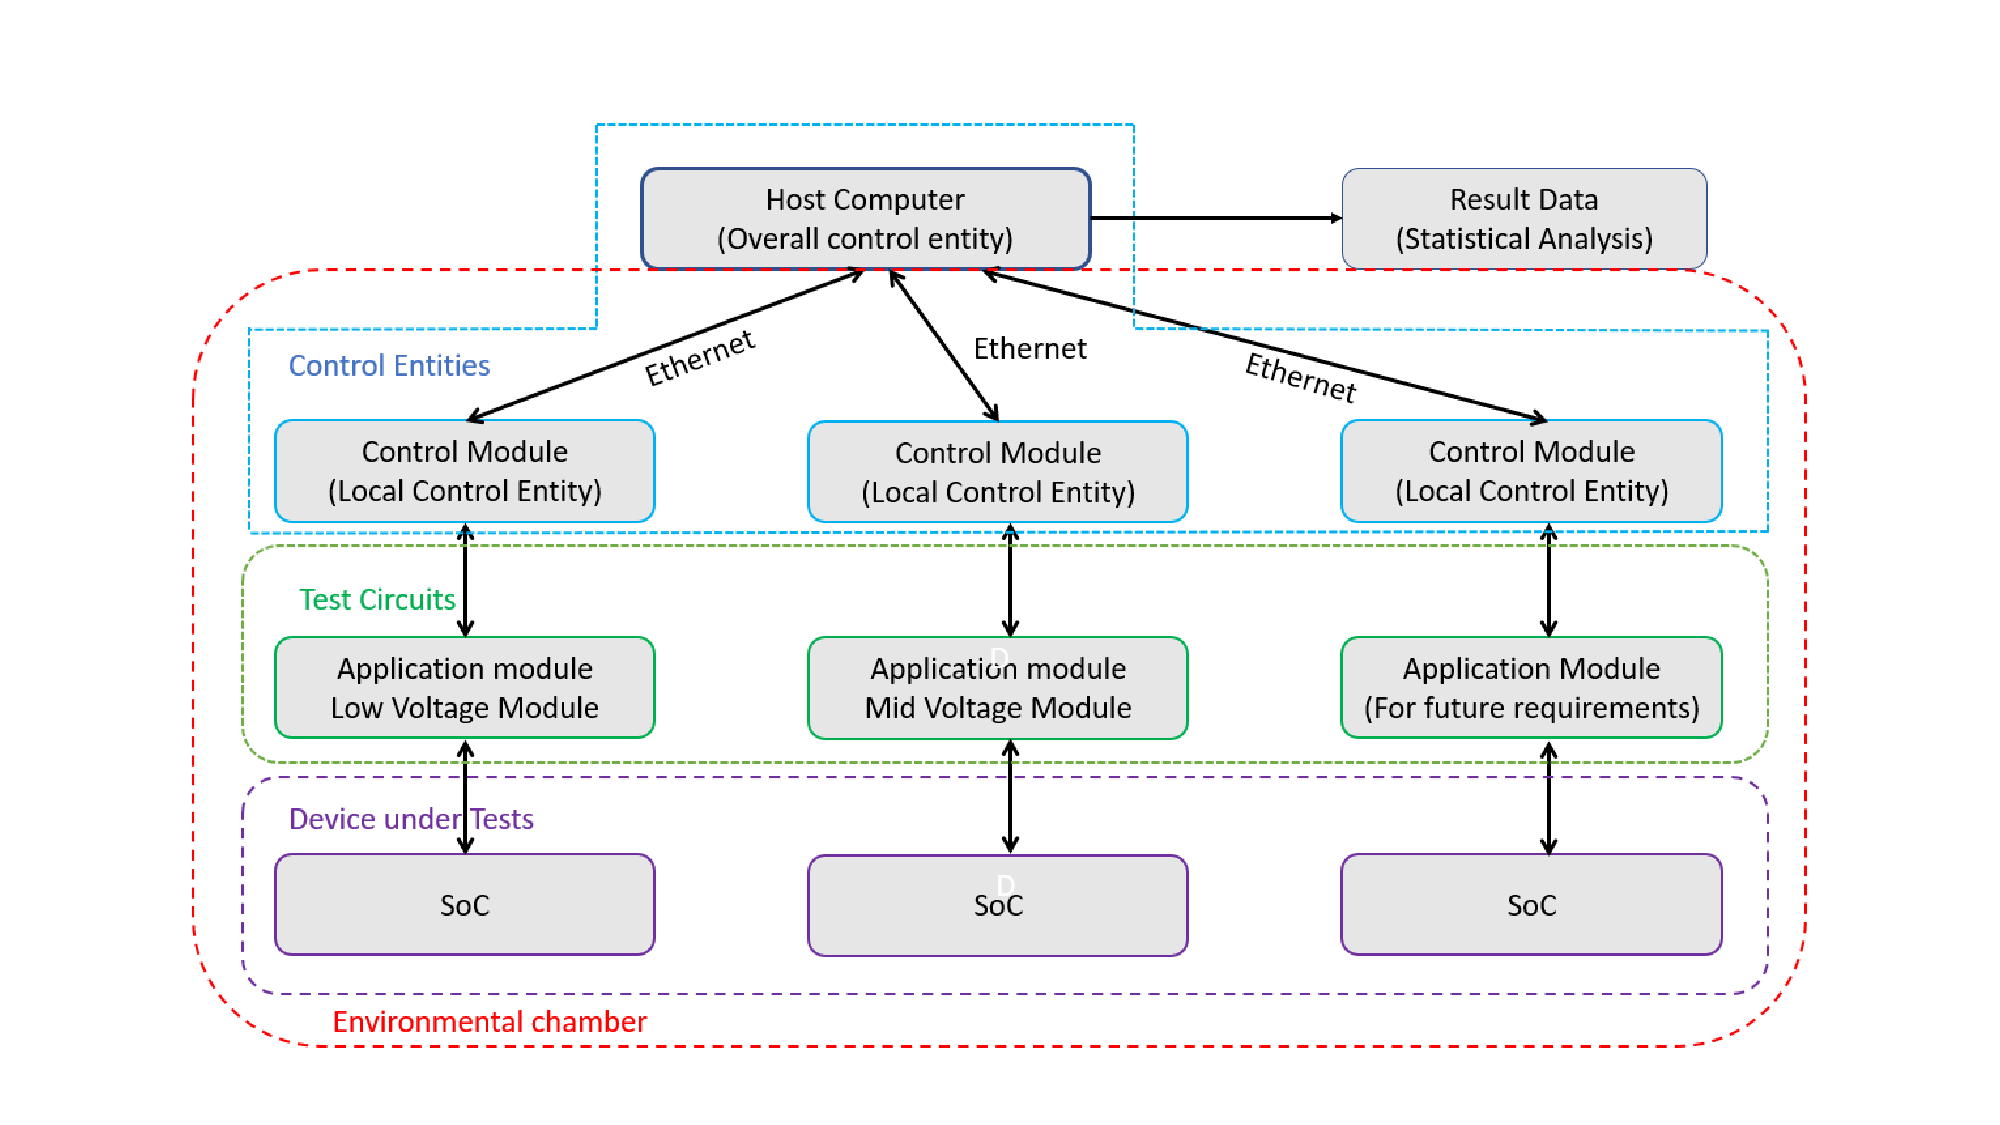
\includegraphics[trim=80 0 0 0, clip, width=170mm]{images/MTS_architecture.pdf}
		\caption{MTS architecture.}
		\label{fig:MTS_image}
		\end{figure}

\begin{figure}
		\centering
		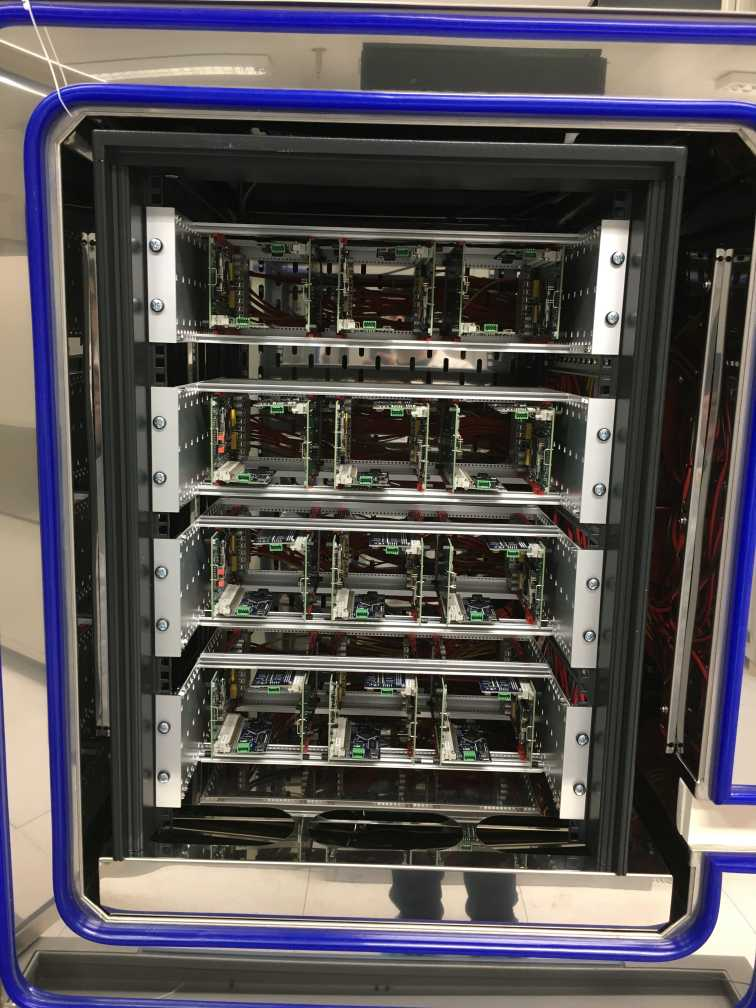
\includegraphics[trim=100 50 0 0, clip, width=65mm]{images/DCDC_System2.jpg}
		\caption{Climate chamber that exerts stress on semiconductor power devices.}
		\label{fig:Climate}
\end{figure}

At KAI, there is a pre-developed modular, flexible and adaptable test system architecture incorporated for reliability stress testing of power semiconductors, which is called \gls{MoPS} architecture~\cite{Steinwender2016}.
This stress test system as shown in \cref{fig:MTS_image} follows a certain flow in delivering a smart approach of executing a reliability stress test on \acrshort{DUT} to estimate their lifetime.
In this stress test system, multiple \acrshort{DUT}s are subjected to stress test patterns under automotive environment conditions.
The MTS architecture is split into two parts, namely the host computer and control module (MicroMoPS). 
The host computer is the central unit system which controls the overall test flow and communicates with the control modules. 
The host computer forwards the test patterns termed as test plans generated by Test Plan Builder~\cite{Plankensteiner2015}. 
Based on the test patterns that are received by control module from a host computer, signals are generated by the control module to provide stimuli to the semiconductor device under test. 
Thereby, the DUT undergoes stress as mentioned in the test pattern. 
The control module further senses the output responses and closes the control loop from a PI controller integrated with the application module, which leads the control module to start recording the measurement parameters of the test. 
The key advantage of \acrshort{MTS} architecture is that there is a total separation of control and measurement part of the test system from the test circuits. 
The test circuits are built within the application module and further, the application module is connected to a semiconductor device under test by a special connector. 
Thus, by the integration of application modules to control modules, it is possible to subject \acrshort{DUT}s into various types of stress tests. 
In order to meet reliability stress testing of power semiconductors under automotive environment conditions, multiple \acrshort{DUT}s and local control modules are attached to the application module and placed inside an environmental chamber as shown in \cref{fig:Climate}. 
These application modules are designed for subjecting \acrshort{DUT}s into specific types of stress test.

Currently, the types of stress tests are:  

\begin{enumerate}
\item Low Voltage Test System: A board called the Buck MoPS is chosen as a \gls{PoL}, which is a DC-DC power converter application. 
The \glspl{DUT} such as power switches are subjected to an application-specific stress test called \emph{power cycling}. 
\glspl{DUT} are heated to reach a temperature between \SIlist{85;125}{\celsius} for consumer devices, \SI{150}{\celsius} for automotive devices and are supplied with a supply voltage that is set to the maximum level which still complies the datasheet specification of DUT. 
Intermittent electronic loads are submitted to \glspl{DUT} which toggle between a high load of {100}{\percent} that nearly reaching \glspl{DUT} to their maximum operating temperature and a low load of \SI{10}{\percent}~\cite{Sleik2016}.  
\item Mid Voltage Test System~\cite{Sleik2018a}: Board such as the \acrshort{PoL} converter is chosen as an application module. 
The \acrshort{DUT}s are power transistors which are subjected to medium voltage stress up to 600V.
\item High Voltage Test System: Devices such as Insulated Gate Bipolar Transistor and \gls{MOSFET} transistors are tested by subjecting to a high voltage of up to 1.5 kV.
\end{enumerate}

The analog measurement data from a DUT is acquired by the data acquisition system of MicroMoPS via the dedicated application module communication channels. 
The analog measurements~\cite{Sleik2018a} such as voltage, current and temperature signals are acquired and go through several stages of attenuation at the application module because of the presence of signal conditioning circuits. 
These signal conditioning circuits are meant for conditioning the measurement data signals into control module specific operating voltage ranges (\SIrange{0}{3}{\volt}).             

\section{MoPS Distributed System}
The Modular Power Stress (MoPS) is a system architecture concept~\cite{Steinwender2013,Steinwender2016} developed to provide a modular infrastructure for customizable stress test applications.
The most essential components of \acrshort{MoPS} system architecture as shown in \cref{fig:MoPS} are: 
\begin{figure}
		\centering
		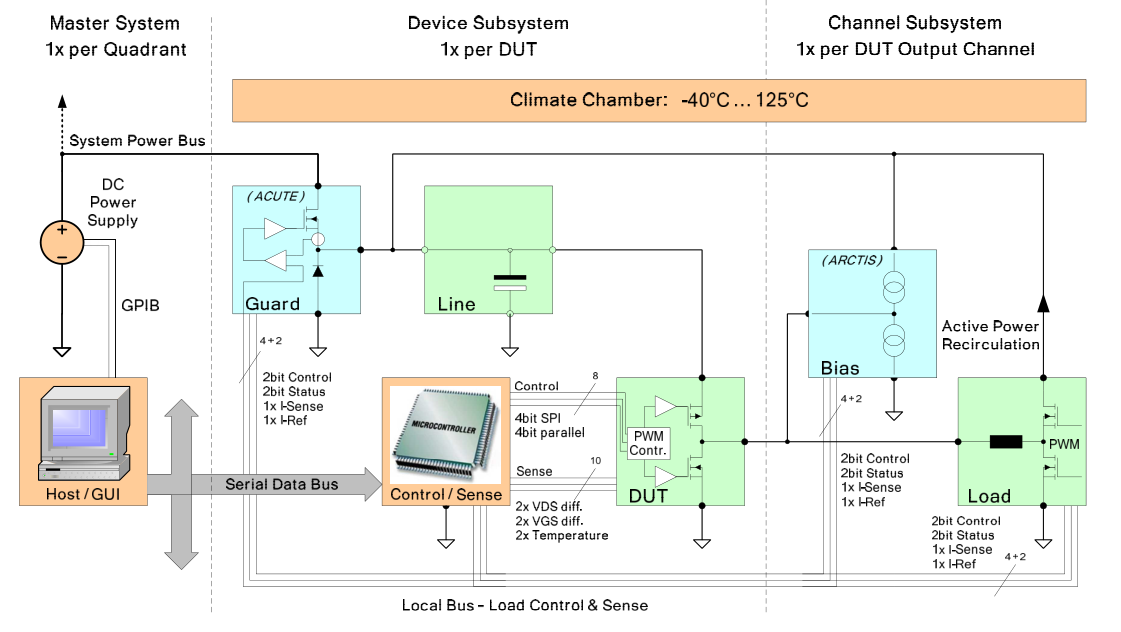
\includegraphics[trim=0 0 0 0, clip, width=\textwidth]{images/MoPS.PNG}
		\caption{Modular Power Stress Distributed system Architecture~\cite{Steinwender2013}.}
		\label{fig:MoPS}
\end{figure}

\begin{description}
  \item[Device subsystem] The components other than control module that are present in the device subsystem act as supporting elements to perform a stress test on a semiconductor device under test. 
  For example, a guard module protects the \acrshort{DUT} from damage by shutting down the power from the control module when there is a device failure. 
  The control module acts as an intermediate agent to trigger application specific stress tests on the \acrshort{DUT}. 
  The control module is situated close to \acrshort{DUT} to establish nearly a lossless one-to-one communication. 
  From the stress tests, the electrical signals that are generated in the \acrshort{DUT} module are measured in the control module via communication channels of the control module.  %And effectively, the local bus(\acrshort{IIC}) is utilised by a control module to detect the UID of associated(better word) application and DUT module. In this thesis, the
  \item[Master system] This is a centralized host, single control entity (see \cref{sec:SAM}) which forwards the stress pattern created by test engineers to a control module (MicroMoPS), to execute stress on the \acrshort{DUT} module. %As, an improvement in exerting the stress pattern to the DUT board, the method of scaling is optimized by including a bit more intelligence to the host computer software i.e SAM, which is discussed in section(refer). 
  \item[Serial Data Bus] This component helps to establish back and forth stress test associated communication between host computer software and the control module. 
  It is also called global bus. 
  Some of the mandatory data exchanges that occur between the host computer software and the control module include: 
	\begin{enumerate}
	\item Reception of test plan by control module from SAM.
	\item Reporting of status and measurement results from control module to SAM via Ethernet. 
	\end{enumerate}
	%Further more set of communications are introduced from this thesis, they are: 
	%\begin{enumerate}
	%\item From this thesis, the UIDs that are detected at the control module, are reported to SAM.
	%\item Based on the UIDs information that SAM has received and oven plan entry given by test engineers(refer test plan builder), respective control module's channels specific scaling value are communicated from SAM to control module, to fit into linear scaling function(refer linear scaling methodologies).
	%\end{enumerate}}
\item[Channel subsystem] The stress test correspondent electronic circuitry namely \acrshort{ARCTIS} is present in this subsystem. An electronic load is driven towards the \acrshort{DUT} via channel subsystem. Also, the real-time controller is part of this system which provides closed loop control logic for the acquisition of the analog measurements.  
\end{description}

\subsection{Hardware architecture}
This section describes the hardware modules of MoPS distribution system.
\subsubsection{MicroMoPS}\label{sec:uMoPS}
The Control module that is used for testing the semiconductor device under test is called MicroMoPS. 
It is a XMC4700~\cite{xmc4700rm2016-RefXMCDatasheet} microcontroller based on the 32bit ARM Cortex-M4 processor core. 
The following are the hardware features that are available in MicroMoPS:

\begin{figure}[htb]
		\centering
		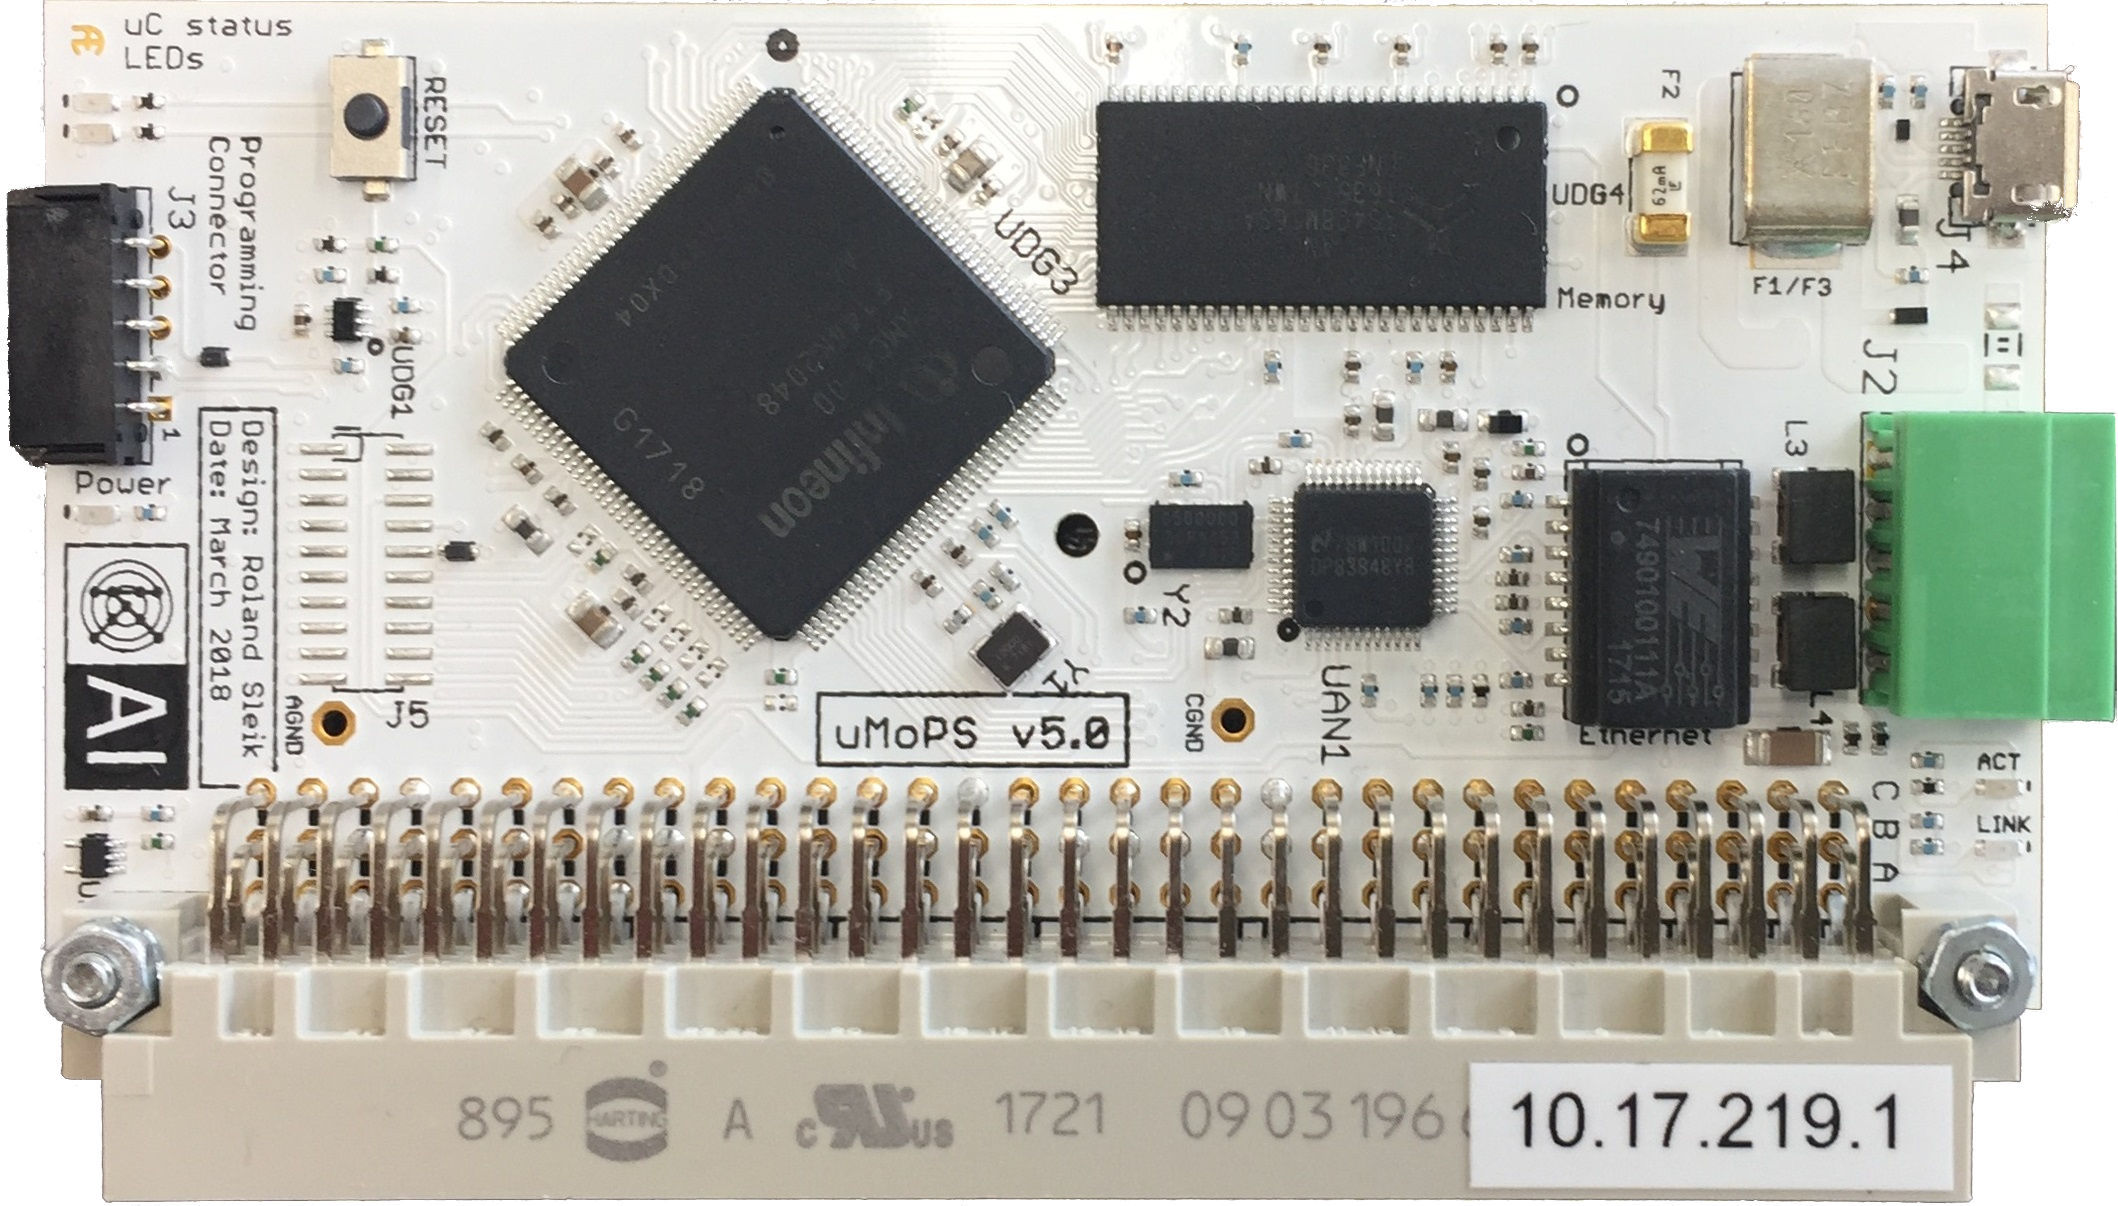
\includegraphics[trim=0 0 0 0, clip, width=120mm]{images/Umopsv5.JPG}
		\caption{MicroMoPS}
		\label{fig:uMoPS}
\end{figure}

\begin{itemize}
	\item Ethernet communication supported with automatic calculation of Medium Access Control (MAC) address deduced from the unique identification number (UID) of the XMC \gls{uC}.
	\item 4 analog input modules capable of acquiring up to 24 input signals with a resolution of 12 bits at rates up to 1.8 MHz.
	\item 4 analog output channels with a 12 bit resolution.
	\item 4 \gls{DSD} channels to gather analog data from galvanically isolated sensors.
	\item 6 \gls{PWM} outputs are divided into 6 units, in which 2 units are provided with an inverted output for half-bridge control.
	\item 1 \gls{SPI} for communicating to a variety of peripherals, such as real-time clocks, memory and control devices such as DAC.	
	\item 1 \gls{I2C} for communicating at low-speed to a variety of peripherals.
			A Key feature of I2C is the capability to control the network of device chips with two \glspl{GPIO} pins.  
	\item 2 \glspl{LED} to indicate run and error states.
	\item 12 \gls{GPIO} pins.
	\item Synchronous DRAM of size 8 MB to store analog measurement data.
	\item Ethernet and \gls{USB} communication interfaces.
	\item Up to 4 software timers of 16-bit width with 1ms resolution for triggering custom events in the test \gls{FSM}.
\end{itemize}

\subsubsection{BuckMoPS}\label{sec:BuckMoPS}
BuckMoPS is the application module which carries the control module - MicroMoPS and DUT - a power switch (IC) to indulge into a low-voltage application stress test system.
BuckMoPS is a DC-DC power stage application.  
The reason behind the addition of an application module together with a control module in the test environment is that it provides a clear separation of stress application from \acrshort{DUT} and control module. 
Also, by introducing an application module into the test system, the \acrshort{DUT}s are subjected to application-equivalent conditions, which helps in the exclusive measurement of power semiconductor device parameters. 
The measurement parameters which are described for the low voltage application stress test system are: input voltage or input current of the \acrshort{DUT}, output voltage or output current of the \acrshort{DUT} and temperature of the \acrshort{DUT}~\cite{Sleik2018a}.   

\begin{figure}[htb]
		\centering
		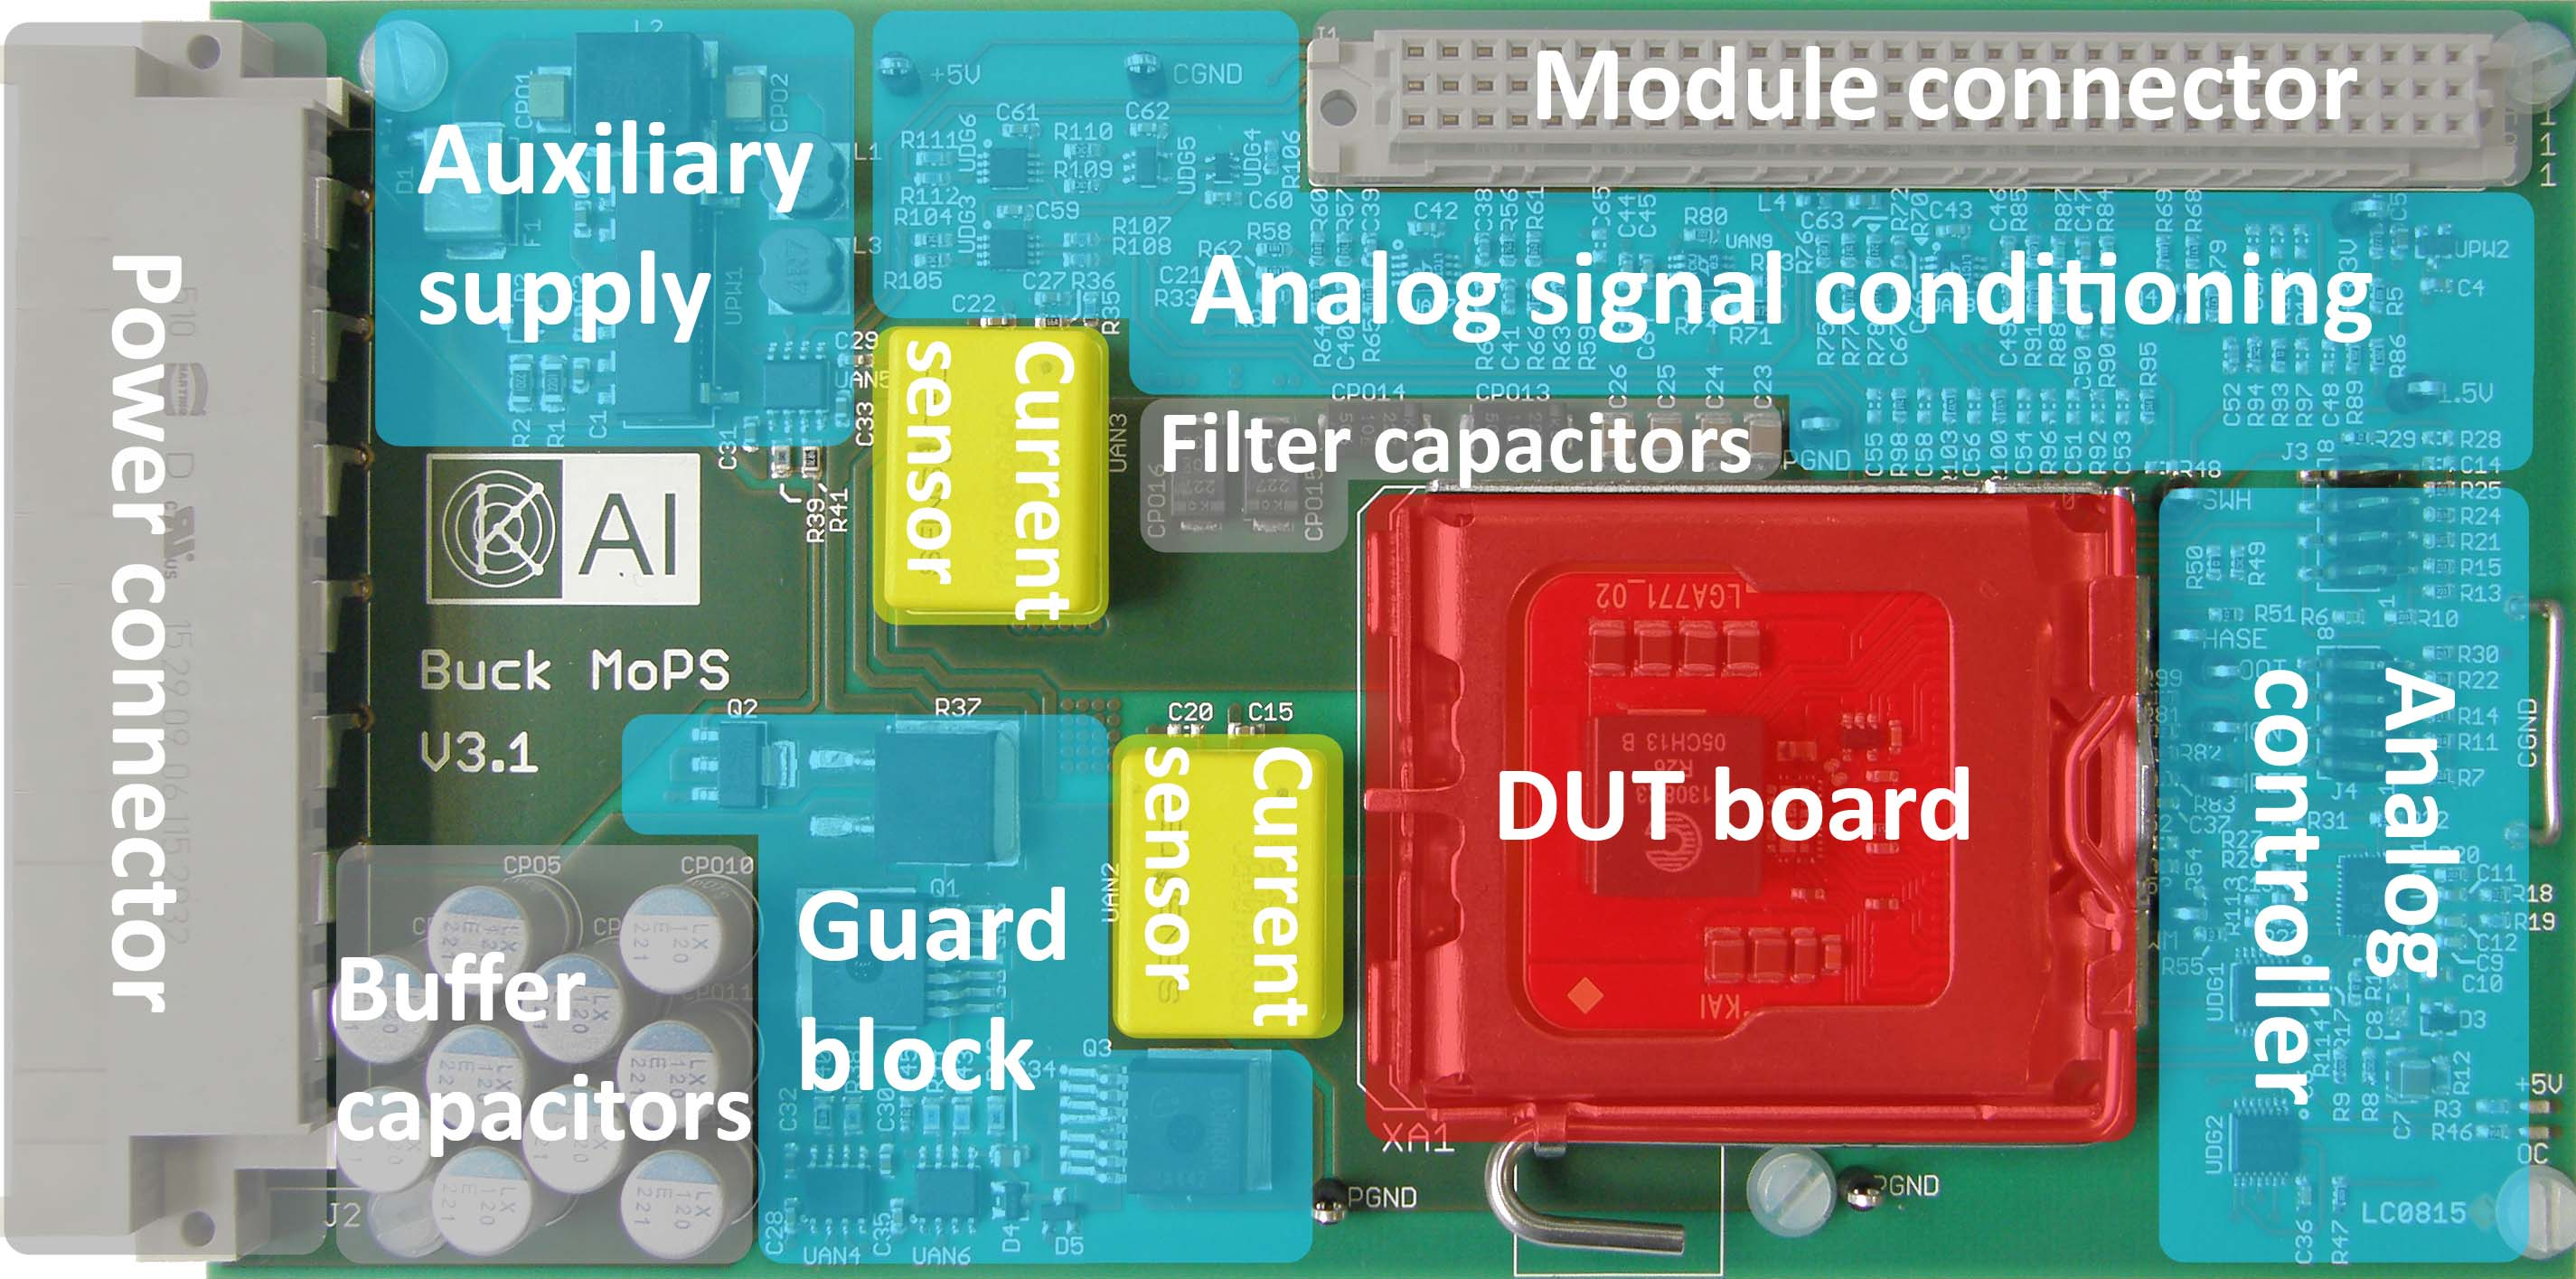
\includegraphics[trim=0 0 0 0, clip, width=\textwidth]{images/Buck_MoPS3.jpg}
		\caption{Low Voltage application board - BuckMoPS.}
		\label{fig:DUT}
\end{figure}

\begin{itemize}[label={}]
\item \textbf{Auxiliary supply:} This module is meant for supplying power to the control module and application module. 
\item \textbf{Guard Block:} This provides smart protection functions that are used to protect the DUT board from over-voltage, which would avoid the damage of the device.
\item \textbf{Analog controller:} This component plays a role in providing a suitable control logic to drive and measure test on DUT board.
\item \textbf{DUT board socket:} This is the area where the DUT board is held and tested.
\item \textbf{Analog signal conditioning:} This component consists of Op-Amps to amplify the signal received from the control module. 
Op-amps are used for conditioning the analog measurement signal i.e. to attenuate analog differential voltage signals into single-ended voltage values that lie within the control module's range. 
\item \textbf{Power connector:} This is the medium by which the power is supplied to application module.
\item \textbf{Buffer and Filter capacitors:} These are useful to support the power supply at high transient events.
\item \textbf{Module connector:} This is the connector that is used to interface control modules.
\item \textbf{Current sensors:} This component is useful for input and output current measurement. 
\end{itemize}

\subsubsection{Device under test}\label{sec:DUT}
The DUT is a pair of \glspl{MOSFET} transistors connected as shown in \cref{fig:BuckMoPS}. 
The Low Voltage application board i.e. BuckMoPS consists of a mentioned \acrshort{DUT}. 
These \glspl{DUT} internally have passive inductors and capacitors to achieve application-equivalent behavior. 
It requires only a \gls{PWM} signal from the control module for the operation of \gls{DUT}.	
\begin{figure}
		\centering
		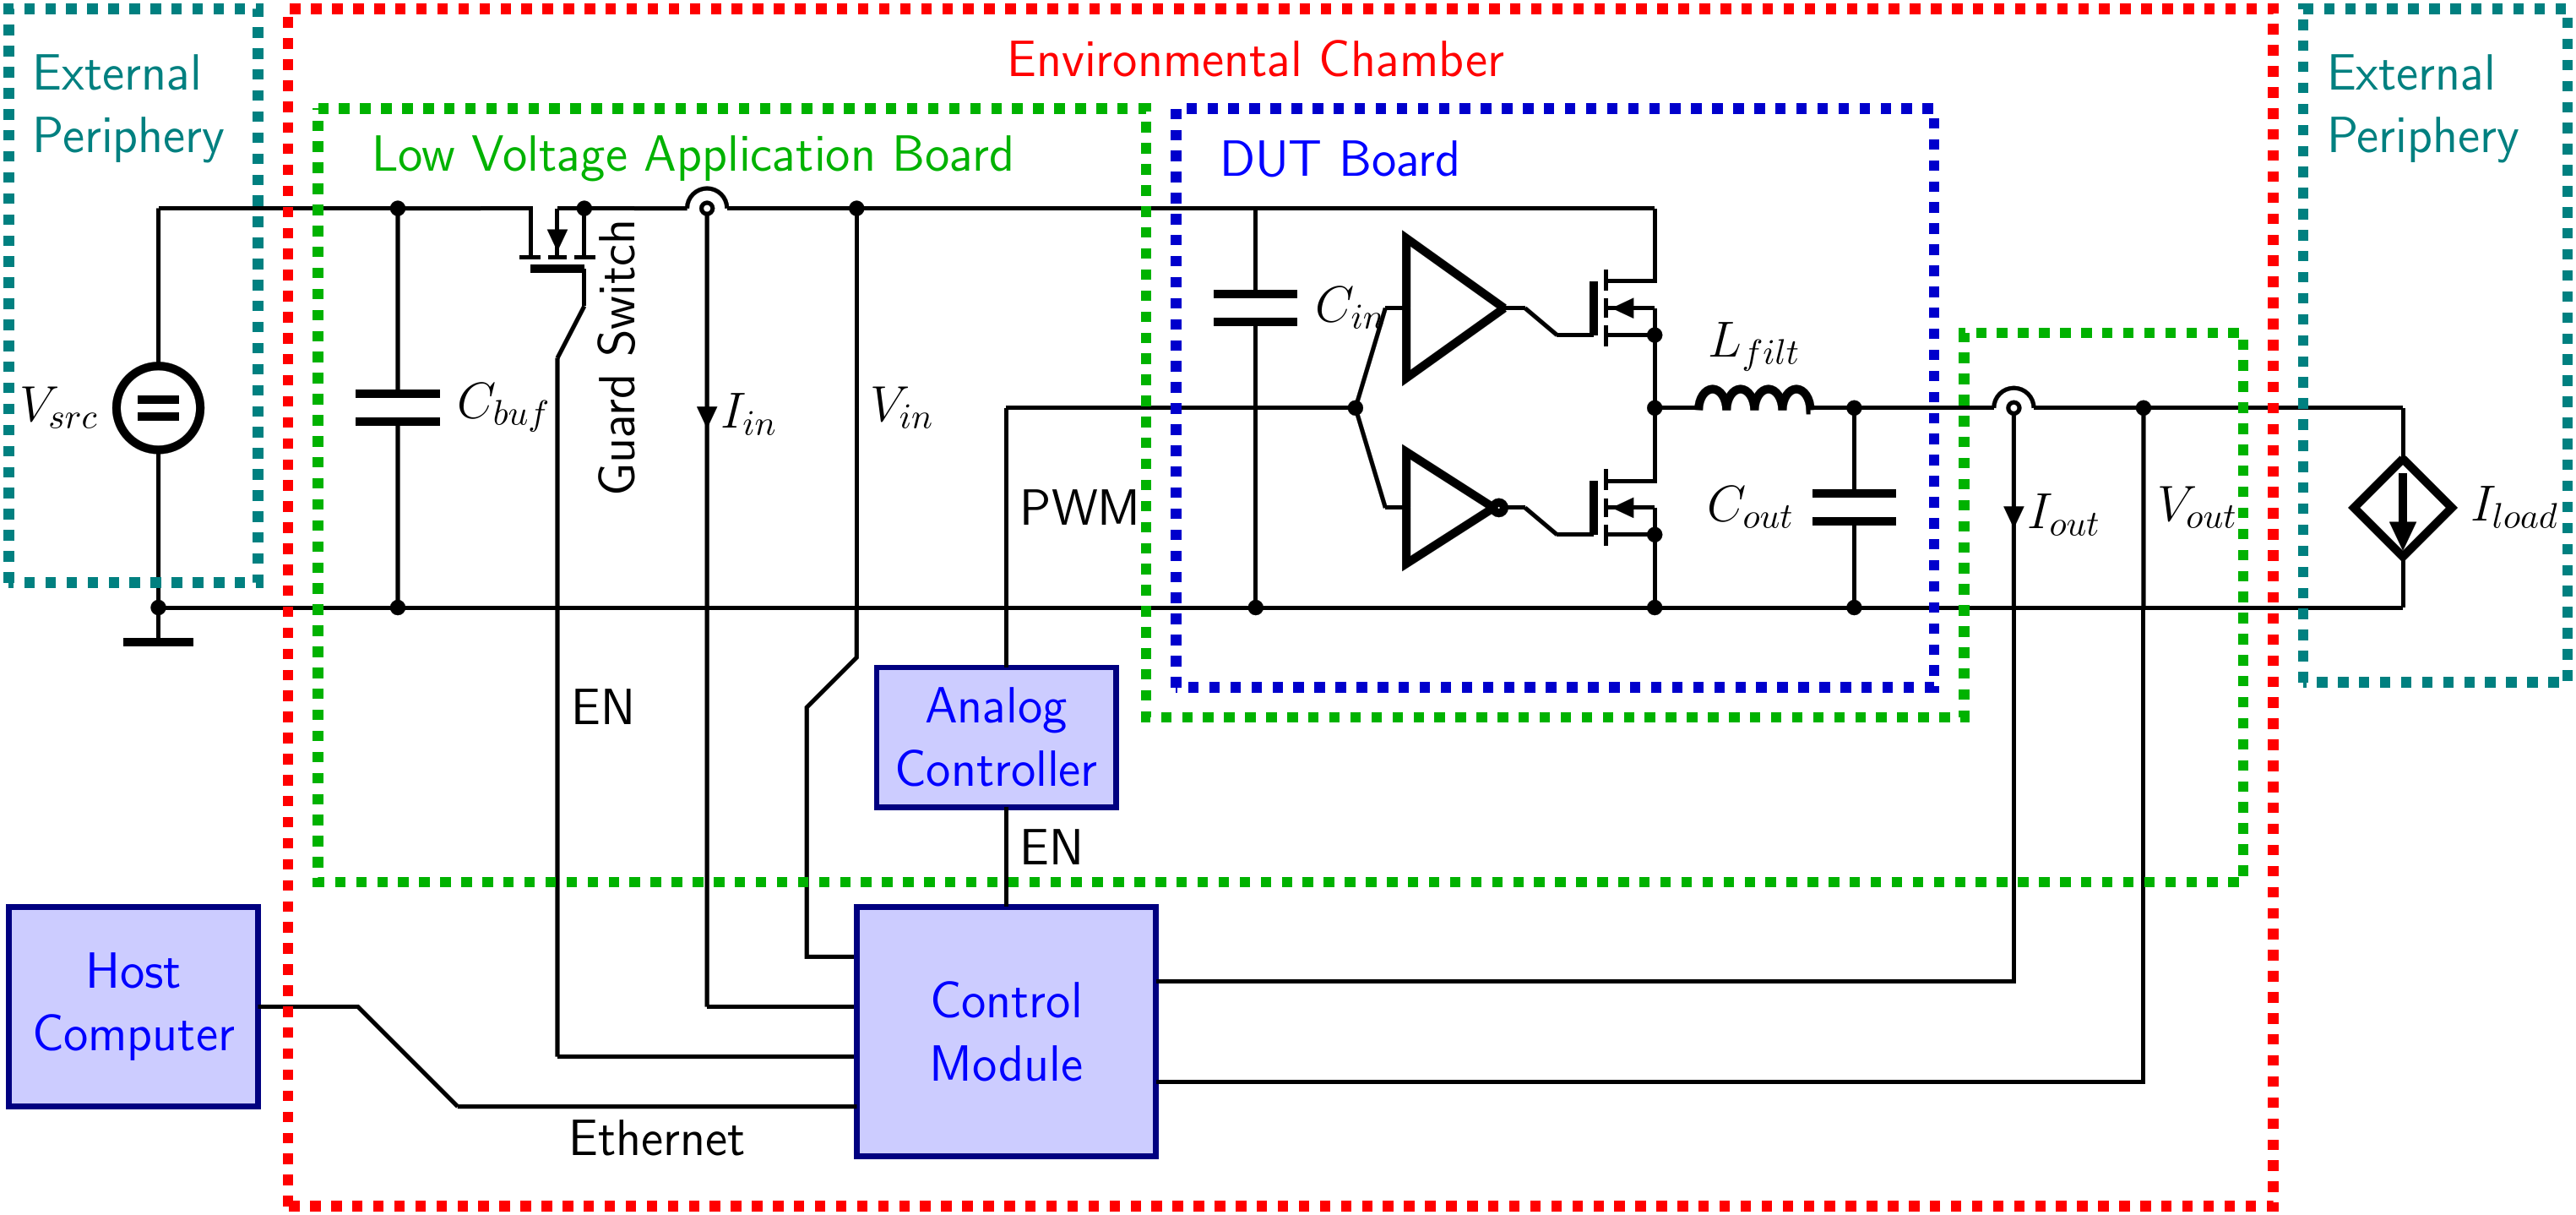
\includegraphics[trim=1370 600 750 100, clip, width=80mm]{images/LV_module_2.png}
		\caption{DUT board plugged to Low voltage application board - BuckMoPS.}
		\label{fig:BuckMoPS}
\end{figure}

\subsection{Software architecture}
This section describes the software layer of MoPS distribution system.

\subsubsection{MoPS-CORE Microcontroller Firmware}\label{sec:CORE}
The MoPS-CORE Microcontroller Firmware is a firmware version of XMC-based microcontroller hardware targets with some CPU resource limitations and memory constraints.
The major handlers that essentially run the entire operation of the MicroMoPS microcontroller are the ones that are included within the main loop. 
By means of measure\_time() handler the time of the main loop is measured for statistical and investigation purposes. 
The handler comm\_handle\_msg() is used in communication between the internal modules of the microcontroller and also to exchange information between the host application i.e. \acrshort{SAM} via Ethernet. 
The handler check\_uplink() is used in testing the connection status between the host and the control module before the test plans are executed on the control module.
Furthermore, the guard\_feed() is a handler that provides a watch-dog guard mechanism, which is a hardware timer capable of resetting the microcontroller, unless it is periodically reset by the software. 
Through the led\_active() handler, the status of the controller is easily detected where there are two \glspl{LED} that are dedicated to give visual indicators to the user about the working state of the controller software. 
Finally, the firmware runs the FSM handler that is developed by test engineers as test procedures and the Lua code that is part of \gls{FSM} diagram is executed to interface the hardware modules of the microcontroller.

%\begin{figure}
%		\centering
%		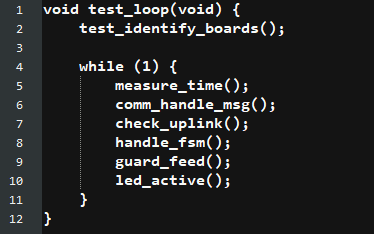
\includegraphics[trim=0 0 50 0, clip, width=100mm, scale=0.75]{images/MoPS_firmware(2).PNG}
%		\caption{MoPS-CORE Microcontroller Firmware}
%		\label{Oven plan window}
%\end{figure}

%\begin{listing}[htp]
%	\inputminted[frame=single]{C}{src/test_loop.c}
%	\caption{MoPS test loop}
%	\label{lst:3-test-loop}
%\end{listing}

\lstinputlisting[frame=single, label=lst:3-test-loop, caption=MoPS test loop, firstnumber=1]{src/test_loop.c}

There are three essential components that are associated to MoPS-CORE Firmware, they are: 

\begin{description}
	\item[Electronic Data Sheet] The \gls{EDS} is the configuration information of control modules that are necessary for performing tests.
	This configuration information includes Hardware version, peripheral information, and device scaling parameters.
	 Fundamentally, the EDS is a JSON string, which is generated upon microcontroller booting. 
	 The microcontroller firmware uses the pre-defined compiled hardware configuration to generate the JSON string. 
	 After the generation of \gls{EDS}, the same is uploaded to the MoPS project web server by SAM so, that other MoPS applications can access the information. 
	%In this work, slight modifications are done in generation of ai MoPS module instance of EDS, in order to facilitate the creation of "scaling.json" in MoPS web server. This "scaling.json" further helps SAM to understand about the expected stress test scenario that needs to be performed and to adjust the scaling parameters in control module to perform linear sclaing. Also, ai communication module of MoPS hardware configuration is extended to enable the operation of linear scaling to process the digital representaion of stress measurements.}     
	
	\item[MoPS web server] The MoPS web server is the server software dedicated for storing Hardware information of the MicroMoPS and delivering Hardware information of the MoPS microcontroller to the corresponding host software application such as TestPlan Builder. 
	 
	\item[Lua interpreter] The Lua interpreter~\cite{Ierusalimschy1996a,Steinwender2015} is to provide flexibility to the hardware designers and product engineers of the company in configuring a test sequence directly without having to deal with the low-level programming of microcontrollers. 
	A set of Lua commands are available to provide a hardware interface and they are simple to use. 
	These Lua commands contain the implementation of custom modules and hardware access routines. 
	They access hardware modules via defined C-APIs. Each Lua command (enclosed within FSM) present in the test plan accesses it's corresponding C-\gls{API} from the Lua space of MicroMoPS firmware and thus, allows the MicroMoPS to execute the entire test plan.
\end{description}


\subsubsection{Software Architecture for MoPS}\label{sec:SAM}
Software Architecture for MoPS is a host layer software~\cite{Steinwender2016} developed using LabVIEW.
This software is designed for test engineers to perform any type of stress testing from their respective host computers.
The stress tests are applied by loading a test plan into SAM software. 
This software makes use of the Actor framework~\cite{ActorFramework2012} of LabVIEW to essentially create multiple independent software agents called as Actors. 
These actors have a separate GUI window displaying their concerned attributes. 
Furthermore, these actors also run some tasks in the background and accordingly their corresponding GUI is refreshed and displayed to provide test engineers a user-friendly interface to interact with. 


\begin{figure}
		\centering
		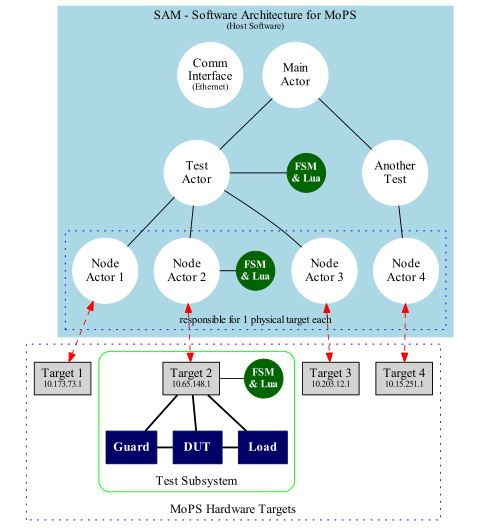
\includegraphics[trim=0 0 0 0, clip, width=80mm]{images/SAM.JPG}
		\caption{Software Architecture for MoPS}
		\label{fig:SAM}
\end{figure}

SAM is organized in a hierarchical manner as shown in the \cref{fig:SAM} where each of these software agents is meant for particular tasks that are fundamentally connected to a target system and responsible for the acquisition of measurement of electrical characteristics of semiconductor power device such as voltage, current, and temperature. 
SAM also facilitates in applying stress to \acrshort{DUT} via control module and to automate the MicroMoPS related host software functionalities.

The Actors that play a major role in the entire operation of SAM are:
\begin{itemize}[label={}]
\item \textbf{Main Actor} This actor is initiated as soon as the SAM application begins to run and during the start-up of this application, the associated child actors i.e. log actor and communication interface are initialized. 
The Main actor is a root actor that is responsible for facilitating the coordination between its sibling actors using queues of LabVIEW's Actor Framework.  

\item \textbf{Log Actor} This actor is used by every other actors to print and log error messages at log actor's \gls{GUI} display window of SAM. 
Thereby, these messages help SAM users and developers to identify and fix bugs that arise while reconfiguring or extending the SAM software.    

\item \textbf{Communication Interface} The Communication interface deals with sending messages to and receiving messages from the control modules via the Ethernet or \acrshort{USB} interface.
 
\item \textbf{Node Actor} The Node actor is responsible for managing a hardware target that is connected to a host computer. 
In the operational case of SAM, the moment the hardware target is connected to SAM, the instance of the hardware node is created and the hardware node's \gls{GUI} window is counter created to display the hardware node's corresponding attributes. 
The GUI of the Node Actor displays information about the node and the test. 
Measurement data acquired by the hardware target is also viewed in this actor. %In this work, the UIDs that are reported from the hardware target is resolved with the webserver generated "boards.json" file to fetch the relevant board names as described in section and displayed in the node actor's GUI window as shown in the figure. From this actor, the test plans are loaded by test engineers. These test plans are created using Test plan builder. And these test plans after loaded to the SAM, are verified for their correctness using Test plan checker. And in the error free case, these test plans are used in control module to subject DUT into application-specific stress as defined in the test plan. These test plans are described in the section.  In this thesis, the board names that are extracted after the resolution of UIDs from "boards.json" are subsequently verified with the oven plan file, to rest assure that the board combinations that are selected in oven plan entry by test engineers match the board names that are fetched from "boards.json". After, succesful verification, the respective control module, application module and DUT module combination is searched from the "scaling.json" to filter the scaling values. The idea of "scaling.json" is to store, every combination of application, control and DUT modules that correspond to the boards that are part of either of available stress test applications(as described in) and also the meaningful information of this board combination i.e respective control module's channels and their scaling parameters. In this work, since the Low voltage application system is the stress test application that is chosen, boards such as BuckMoPS, BuckVoyager and MicroMoPS combination is searched for. And once when the combination is found from the lookup table, it's associated channel names and their scaling values are extracted/filtered. These channel names and scaling values are further communicated to a particular method of the control module's firmware thereby, these scaling values are adjusted to linear scaling function.}

\begin{figure}[hbt]
		\centering
		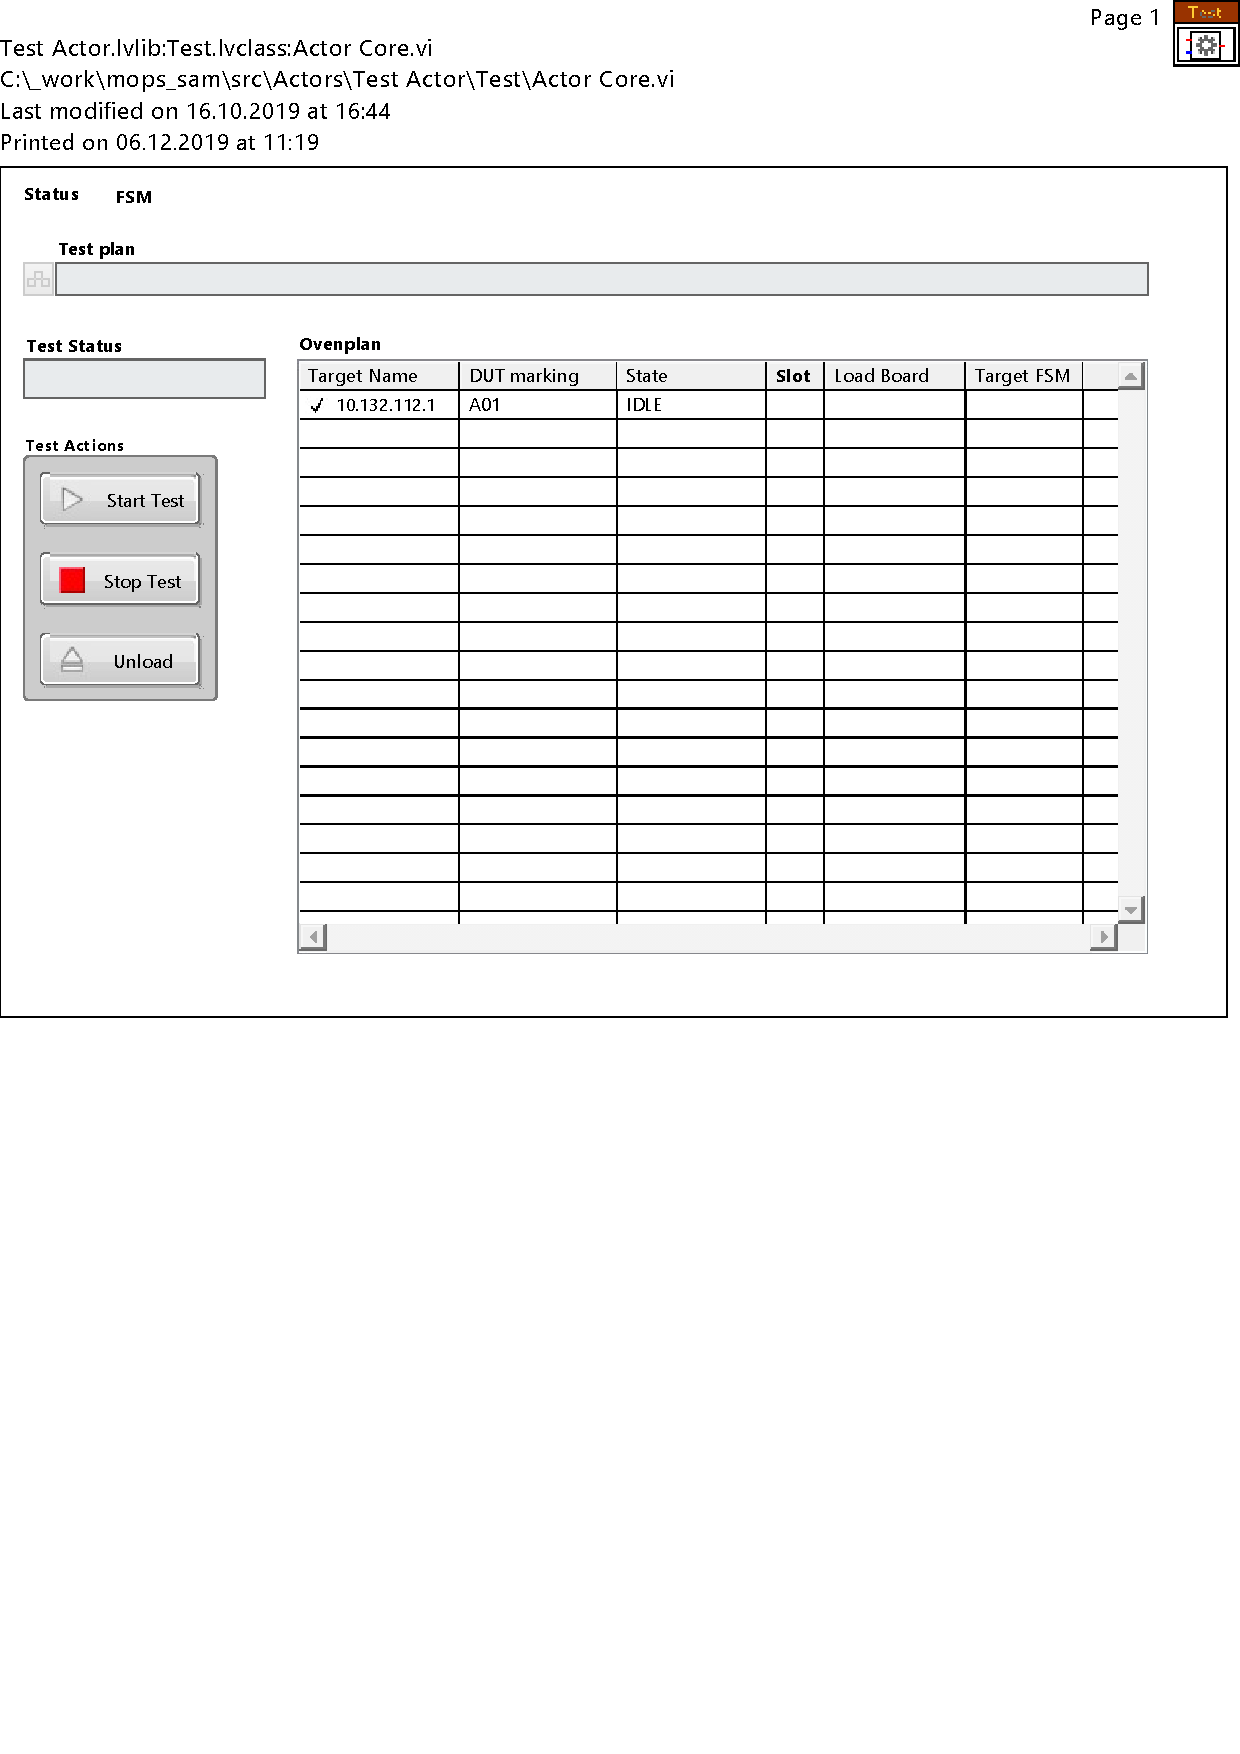
\includegraphics[trim=0 400 0 100, clip, width=100mm]{images/Testactor.pdf}
		\caption{Test Actor}
		\label{fig:Test}
\end{figure}

\item \textbf{Test Actor} Test actor provides a GUI platform to display the test status to the user and also provides the interface to send test events to the control module. 
GUI display of Test Actor is as shown in the \cref{fig:Test}. 
To start the test, "start" is the event that is executed. 
To stop the test, "stop" is the event that is executed. 
Once, when the test starts running, the analog measurements can be acquired by an event "meas", which is executed from the \gls{FSM} window of Test actor. 
Test actor in much general sense executes the finite state machine given in the test plan (see \cref{sec:TP}).    
\end{itemize}

\begin{figure}[hbt]
		\centering
		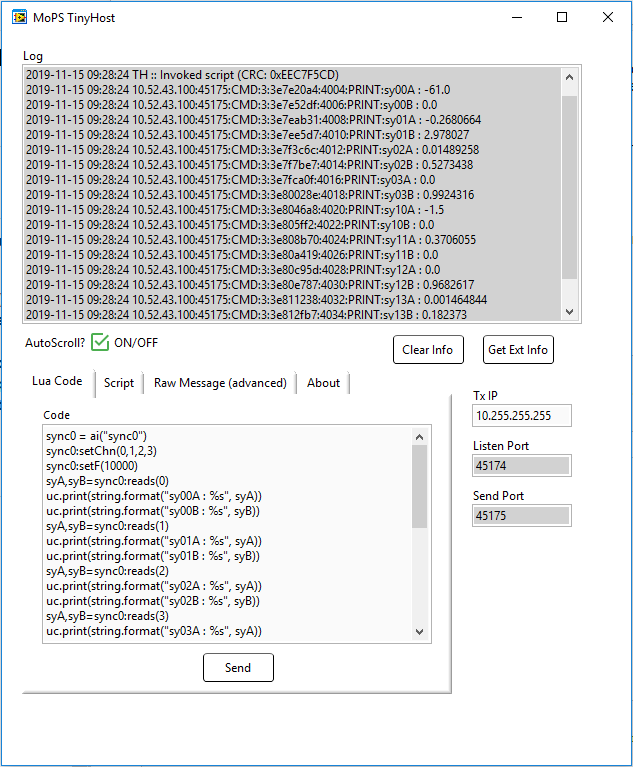
\includegraphics[trim=0 0 0 0, clip, width=100mm, scale=0.75]{images/Tinyhostaichannels.PNG}
		\caption{TinyHost application}
		\label{fig:tinyhost}
\end{figure}


\subsubsection{TinyHost}\label{sec:TinyHost}
A small application called TinyHost exists to test the communication interface of the MicroMoPS and also to send messages to the hardware targets. 
Through, this application the messages can be sent to the hardware targets manually and thereby, commands that are part of Lua interpreter which are present in the microcontroller's firmware are executed. 
To get a sense of TinyHost's purpose, an example of one of the tests that are performed during this thesis is considered. 
In this work, to test the functionality of hardware target's analog input communication modules and their channels' value (see \cref{sec:Channels}), Lua code (see \cref{sec:Lua}) is written to invoke Lua commands that are present at the Lua space of microcontroller's firmware, as shown in the \cref{fig:tinyhost}. 
Subsequently, the result is displayed on the log field of the TinyHost as shown in the \cref{fig:tinyhost}. 
\subsubsection{Test Plan Builder}\label{sec:TP}
Test plan builder~\cite{Plankensteiner2015} is an application used to create a test plan in the form of a \acrshort{FSM} diagram where each state of the FSM diagram is fundamentally a set of Lua commands that are defined in the microcontroller's firmware. 
Test plan builder also downloads the \acrshort{EDS} from the MoPS web server to know the details of the latest hardware configuration of MicroMoPS. Consequently, from the knowledge of hardware configurations, Test-plan builder enables the test engineers to create a test plan. 
The development procedure of test plans and the syntactic rules that are applicable to successfully build test plans are described in detail in Plankensteiner's Master thesis~\cite{Plankensteiner2015}. 
EDS configuration information is necessary for verifying the respective hardware capabilities before a test starts. 
The Test-Plan Builder requires this information to provide knowledge to test design engineers about the available hardware and software modules that could be used in creating test plans. 
A sample of the test plan is as shown in the \cref{fig:Testplan builder}. 
In principle, there are two sections in the layout of a Test plan tab of Test plan builder, they are:  

%Test-Plan builder is the application that downloads the new and updated EDS files from the webserver to validate test plans. 

\begin{figure}[hbt]
		\centering
		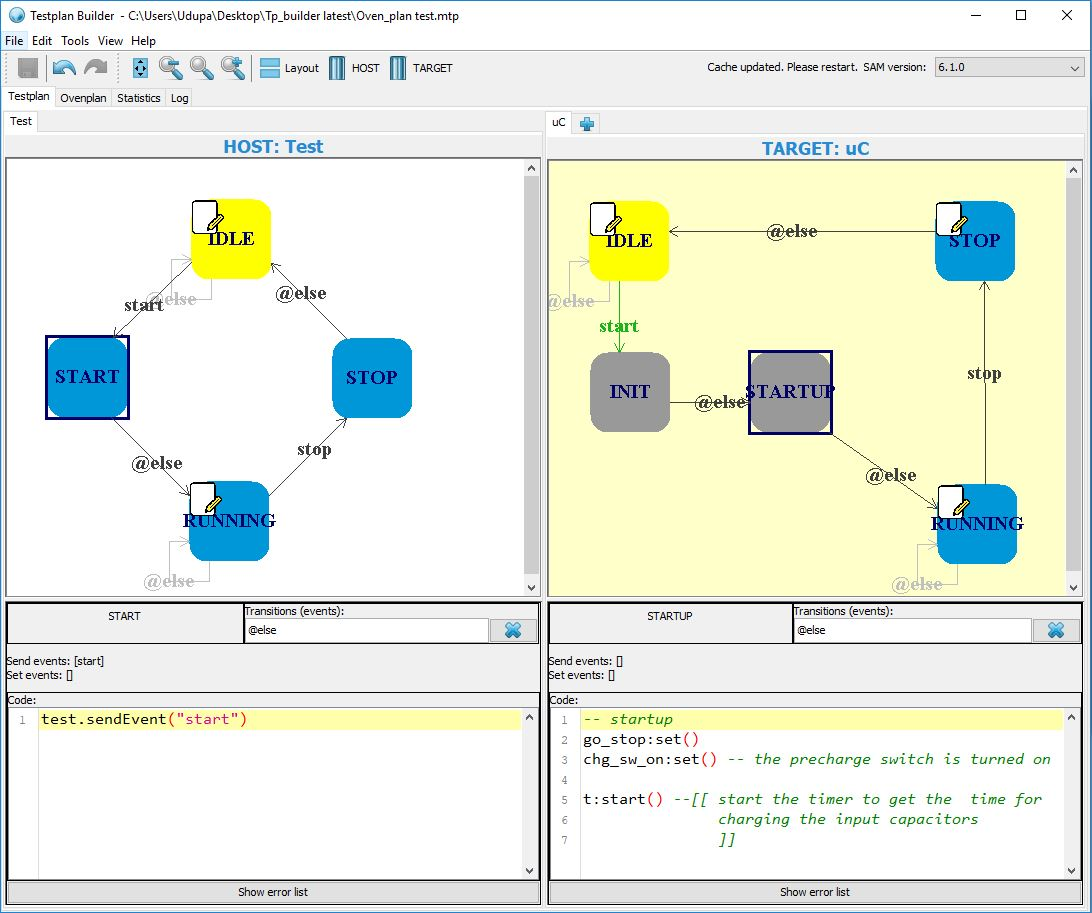
\includegraphics[trim=0 0 0 0, clip, width=150mm]{images/TPbuilder.JPG}
		\caption{Test plan builder application}
		\label{fig:Testplan builder}
\end{figure}

\begin{figure}[hbt]
		\centering
		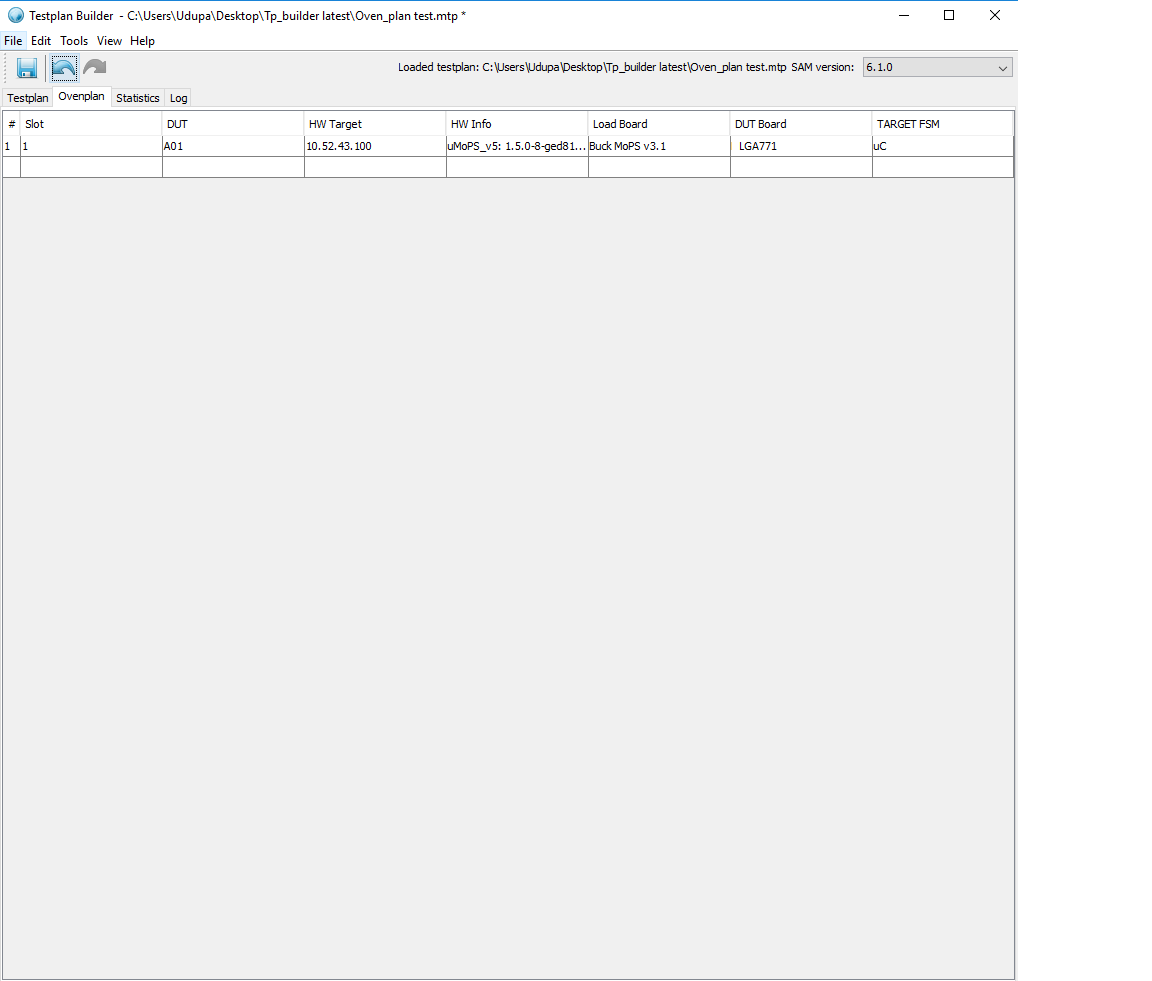
\includegraphics[trim=0 600 0 0, clip, width=\textwidth, scale=0.75]{images/Ovenplan_edited.PNG}
		\caption{Oven plan window}
		\label{sec:Oven plan window}
\end{figure}

\begin{enumerate}
\item \textbf{HOST:} The \acrshort{FSM} diagram in Host is meant for providing control over the operation of the Target FSM diagram. 
As soon as the start button is pressed after loading the test plan to SAM, there occurs a transition from the IDLE state of Host FSM to the START state in test execution. 
This START state machine sends a "start" event to the IDLE state machine of Target FSM which, leads Target FSM to propagate further from the IDLE state.
    
\item \textbf{TARGET:} The FSM diagram in Target is the starting point for the control module to subject \acrshort{DUT} into stress, where the functionality of Target FSM is totally controlled by the Host FSM.
Intuitively, the running of all the state machines of Target FSM except INIT is nothing but the invoking of Lua commands that are specific to microcontroller's firmware modules (\cite{Steinwender2016}, p.39). 
As soon as Target FSM is triggered by Host FSM by receiving a start event, there occurs a transition from the IDLE state to the INIT state in Target FSM. 
Consequently, at INIT a digital stimuli is generated towards the DUT because of the PWM signal from the control module. 
Furthermore, Target FSM reaches to running state which, is an indication that the test is running. 
Finally, the test is stopped by pressing a stop button in SAM, which results in the Target FSM diagram to reach to its IDLE state from any given state.  
\end{enumerate}

%In this work, the more concentration is towards the information that is generated because of the entries that are provided in the oven plan. 
\textbf{Oven plan} The oven plan of the Test plan builder tool provides an interface to select desired DUT, application module and Hardware target. 
Test engineers select the board names based on the stress type they want to perform. 
The selection of boards is done by a drop-down present in the oven plan window of the test plan builder. 
A variant of MicroMoPS (classified by their IP address), Application module and DUT are chosen as shown in the \cref{sec:Oven plan window}.     
The test FSM diagram in the test plan window and hardware selection in the oven plan window fulfills the protocol of the creation of the test plan. 
Further, to which the test plan is generated as a JSON file. 
The JSON file is loaded to SAM to execute the stress test. %In the meantime, SAM uses the same JSON file counterpart to fetch the board names that are selected by test engineers.

%In addition to the fundamental modules that drive microcontroller firmware, another handler is developed such as test\_identify\_boards() to reach one of the milestones of this thesis.


%To consider explaination in terms of ADC conversion by referring Versatile Analog to Digital Converter.
\subsection{Measurement environment of MoPS}\label{sec:ME}

This section describes the measurement data acquisition system of MicroMoPS, measurements communicating channels of MicroMoPS, signal conditioning circuits present in the measurement environment and processing concepts. 

\subsubsection{Measurement data acquisition of MicroMoPS}\label{sec:DAQ} 
\glsentryfull{DAQ} of MicroMoPS is responsible for acquiring, displaying and storing the analog measurements that are obtained from tests. 
The analog measurements such as temperature, voltage, and current of the test are sent to Analog-to-digital converter (ADC) of the MicroMoPS via dedicated analog input channels. 
These measurements that are received at the ADC of MicroMoPS, are sampled and quantized to convert into a certain range of digital values. 
In general, the ADC of a MicroMoPS is of 12 bit resolution, therefore the analog values that are converted into digital values range from 0 and 4095 and represent the microcontroller's specific voltage values range from \SIrange{0}{3}{\volt}. 
These measurements go through some signal conditioning (see \cref{fig:Conditioning}) before they are used by the ADC to perform digital conversion.
The analog measurements that are communicated using analog communication channels are classified into two types: 
\begin{enumerate}
\item \textbf{Single-ended multi-channel measurements:} This type of measurement requires the analog value to be referenced to the well chosen common-mode i.e. Ground.
\item \textbf{Differential measurements:} This type of measurement does not have common-mode reference but have a difference in analog value between the two input signal leads.
\end{enumerate}

The communication channels which conduct analog measurements follow a certain hierarchy in their design (see \cref{Channels}) and these measurements are converted from differential measurements/single-ended channel measurements to single-ended values by allowing them to go through signal conditioning. 
Because of this, the measurements are achieved in delimiting them into the microcontroller operating voltage range i.e., \SIrange{0}{3.3}{\volt}.

\subsubsection{Channels hierarchy and their purpose}\label{sec:Channels}
Analog-to-digital conversions in MicroMoPS can be executed in two modes. They are:
\begin{enumerate}
\item \textbf{Synchronous mode} - Channels belonging to a synchronous group can do an analog-to-digital conversion in parallel as the ADC kernels of these channels are synchronized with each other.  
\item \textbf{Scan mode} - Channels belonging to the scan group follow a configurable linear sequence that allows the dedicated channels to do analog-to-digital conversion one after another.
\end{enumerate}
\begin{figure}[hbt]
		\centering
		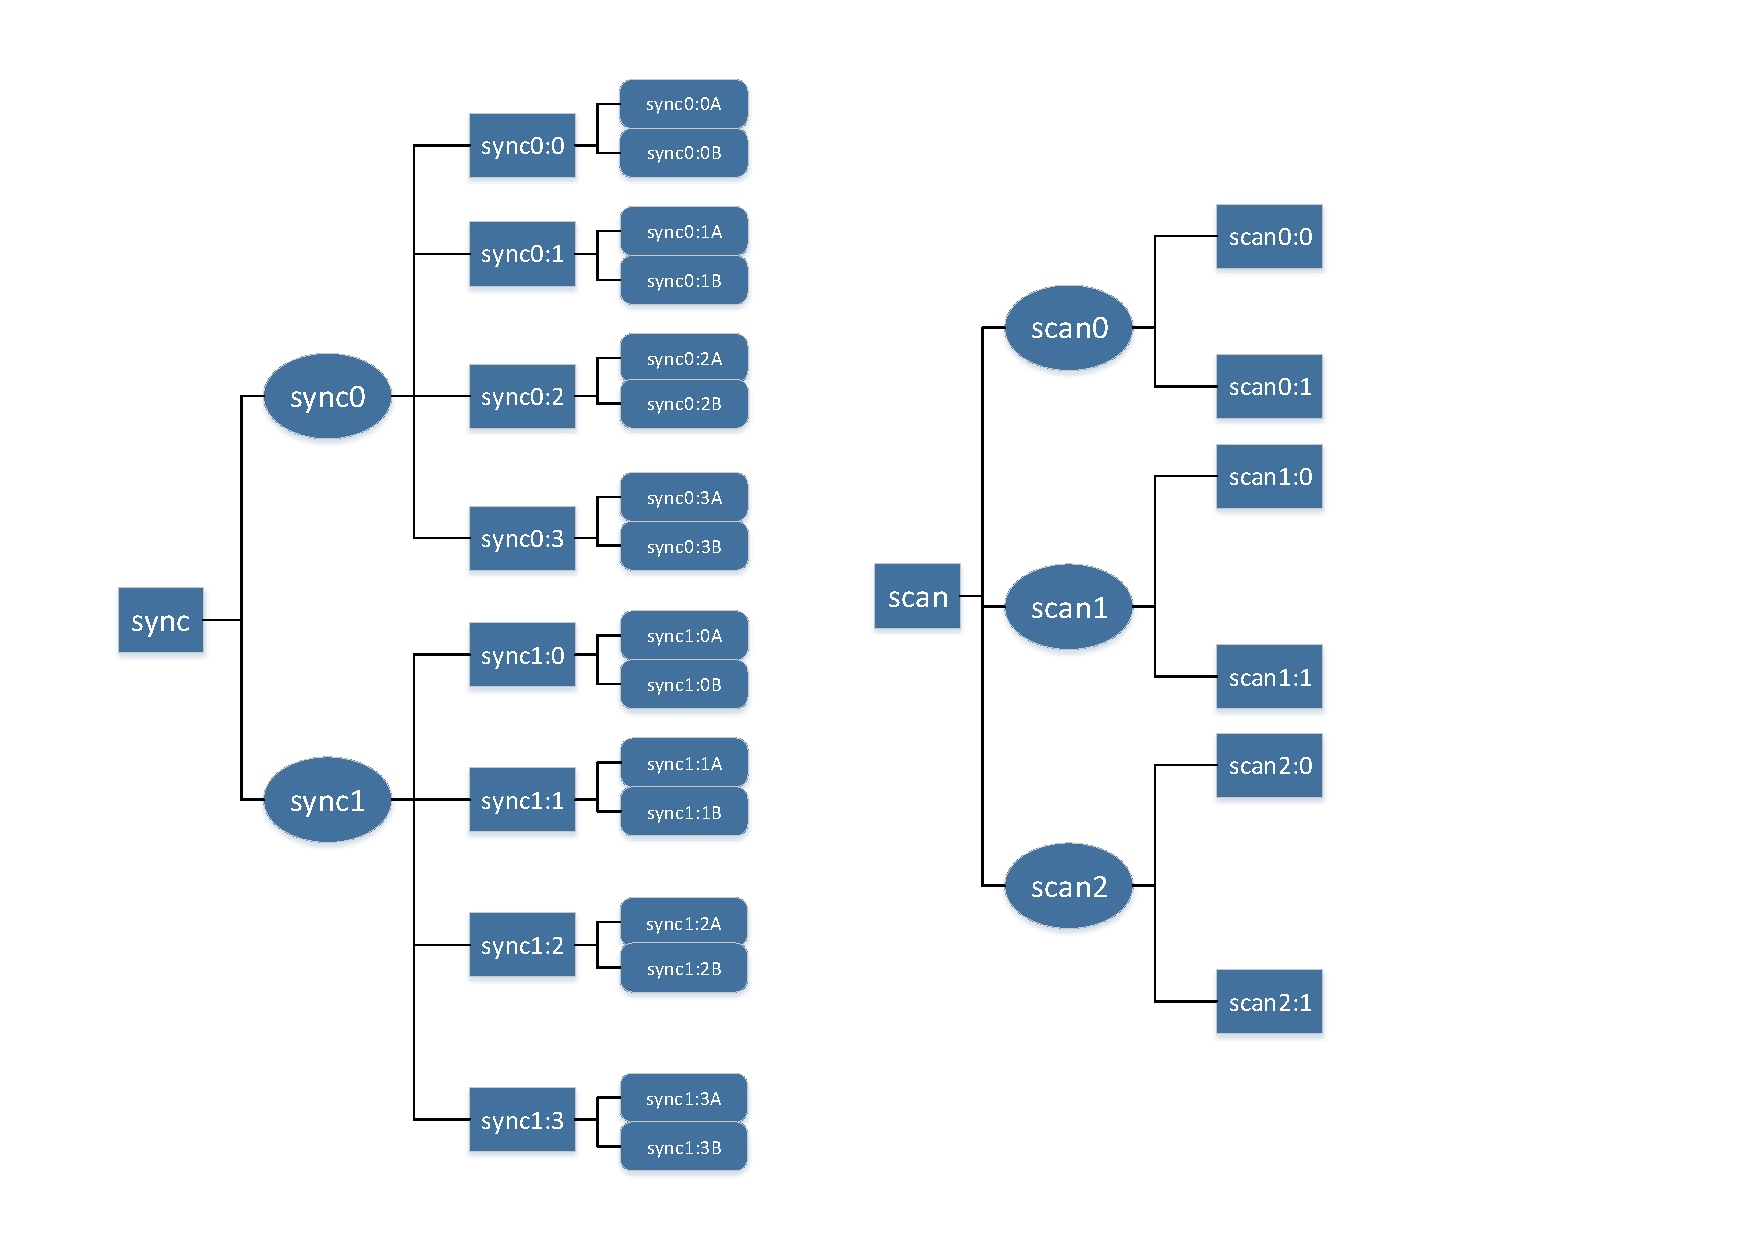
\includegraphics[trim=0 0 50 0, clip, width=125mm, scale=0.75]{images/channels_hierarchy.pdf}
		\caption{Channels hierarchy}
		\label{Channels}
\end{figure}
With respect to the modes of analog-to-digital conversion, there are dedicated channel modules such as sync0, sync1, scan0, scan1, and scan2. The mentioned channel modules as they are named, correspond to synchronous and scan conversion modes. These channel modules are further classified as follows:
\begin{enumerate}
\item \textbf{sync[0,1][0,3]B} - Unipolar Analog-to-Digital conversion synchronous channels, where first index, i.e, [0,1] represents the module number, second index, i.e, [0,3] represents the module's specific channel number and third index represents the channel's specific group name. 
The group name assigned to this channel is 'B'.    
\item \textbf{sync[0,1][0,3]A[N,P]} - Bipolar Analog-to-Digital conversion synchronous channels, where first index, i.e, [0,1] represents the module number, second index, i.e, [0,3] represents the module's specific channel number and third index represents the channel's specific group together with the polarity, i.e, -/+ of the elelctrical signal. The group name assigned to this channel is 'A'.
\item \textbf{scan[0,1,2][0,1]} - Analog-to-Digital conversion scan channels, where first index, i.e, [0,1] represents the module number, second index, i.e, [0,1] represents the module's specific channel number.
\end{enumerate}

The Differential Voltage measurements such as Switch Node Voltage (Vswh),  Measurement voltage from Auxiliary MicroMoPS node 1 (Aux1), IC current monitor (Imon), Converter input voltage (Vin) and Converter output voltage (Vout) are acquired via bipolar Analog-to-Digital conversion channels i.e. \textbf{sync[0,1][0,3]A[N,P]}.
Aux1 and Aux2 are the auxiliary MicroMoPS that are used to cover multiple functions available on the test device.

The single ended Voltage or Current or Temperature measurements such as Converter input current (Iin), Converter output current (Iout), DUT case temperature (Tc), DUT board temperature (Tbrd), Driver current (Idrv), Driver Voltage (Vdrv), IC current monitor (Imon) and IC temperature monitor (Tmon) are acquired via unipolar analog-to-digital conversion synchronous channels i.e. \textbf{sync[0,1][0,3]B}. 

The above measurement parameters are part of the Low Voltage MTS environment~\cite{Sleik2018a}.

\subsubsection{Analog signal conditioning circuits}\label{sec:asc}
To most of the measurement signals, the analog signal conditioning circuit setting is merely the differential amplifier with a series resistor and standard voltage divider circuits convention as shown in the \cref{fig:Conditioning}. This signal conditioning circuit is designed by the hardware designers of KAI.  
\begin{figure}[htb]
		\centering
		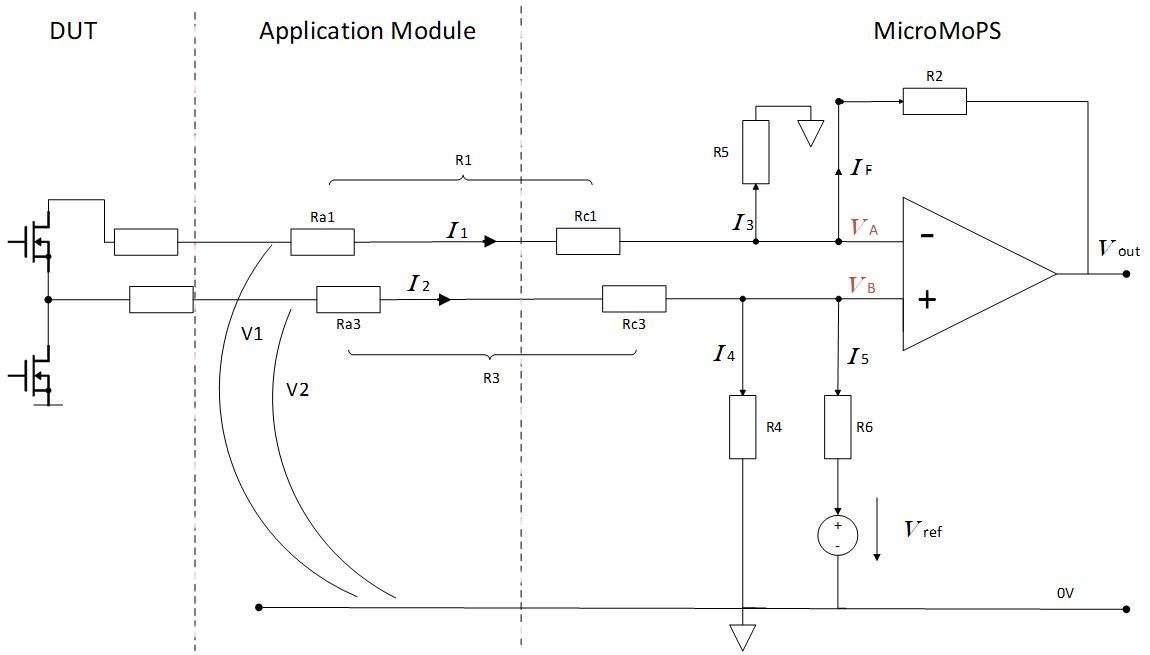
\includegraphics[trim=10 0 0 0, clip, width=150mm, scale=0.75]{images/conditioning.JPG}
		\caption{Analog signal conditioning circuit}
		\label{fig:Conditioning}
\end{figure}

Conditioning of the voltage, temperature, and current signals is achieved by using an analog signal conditioning circuit (see \cref{fig:Conditioning}) with some standard component values. 
The analog signal conditioning circuit for \gls{Iin} and \gls{Iout} are placed on the application module and the resulting conditioned signal is directly fed to analog-to-digital converters of the control module. 
The analog signal conditioning circuit for \gls{Vin}, \gls{Vout} and \gls{Imon} are placed on the control module. 
For the DUT case temperature measurement i.e. \gls{Tcase}, the resistive sensor is supplied from a constant current source with a provision of voltage amplification. \gls{Tmon} in an application module to monitor the DUT temperature. 
\gls{Vdrv} in the application module consists of a Voltage divider circuit to drive MicroMoPS. 
Finally, \gls{Idrv} in the application module to supply current to MicroMoPS.

\subsubsection{Processing concepts}\label{sec:Pc}
Finally, in order to convert the digital measurements (representative of the analog measurements of the \acrshort{DUT}) into microcontroller's specific analog values which range from \SIrange{0}{3}{\volt}, the respective digital values need to be processed.
The method of processing digital values is called a scaling function. This scaling function can vary from channel to channel because of the varying microcontroller specific analog value range for particular test measurements. 
For an instance, the microcontroller specific analog value range for the channel \textbf{sync[1][0]A} ranges from \SIrange{-1.5}{+1.5}{\volt} whereas, the microcontroller specific analog value bandwidth for the channel \textbf{sync[0][0]B} ranges from \SIrange{0}{3}{\volt}. 
Standard scaling function (see \cref{eq:Scaling}) is used to process the analog measurements.  

\section{State of the art}\label{sec:SOA}
Stress test application on a high level goes at a particular flow. 
This flow essentially provides the state of the art that exists in this stress test environment.
The flow of the stress test as depicted in \cref{fig:SOA} is explained accordingly in steps as follows:   

\begin{figure}[htb]
		\centering
		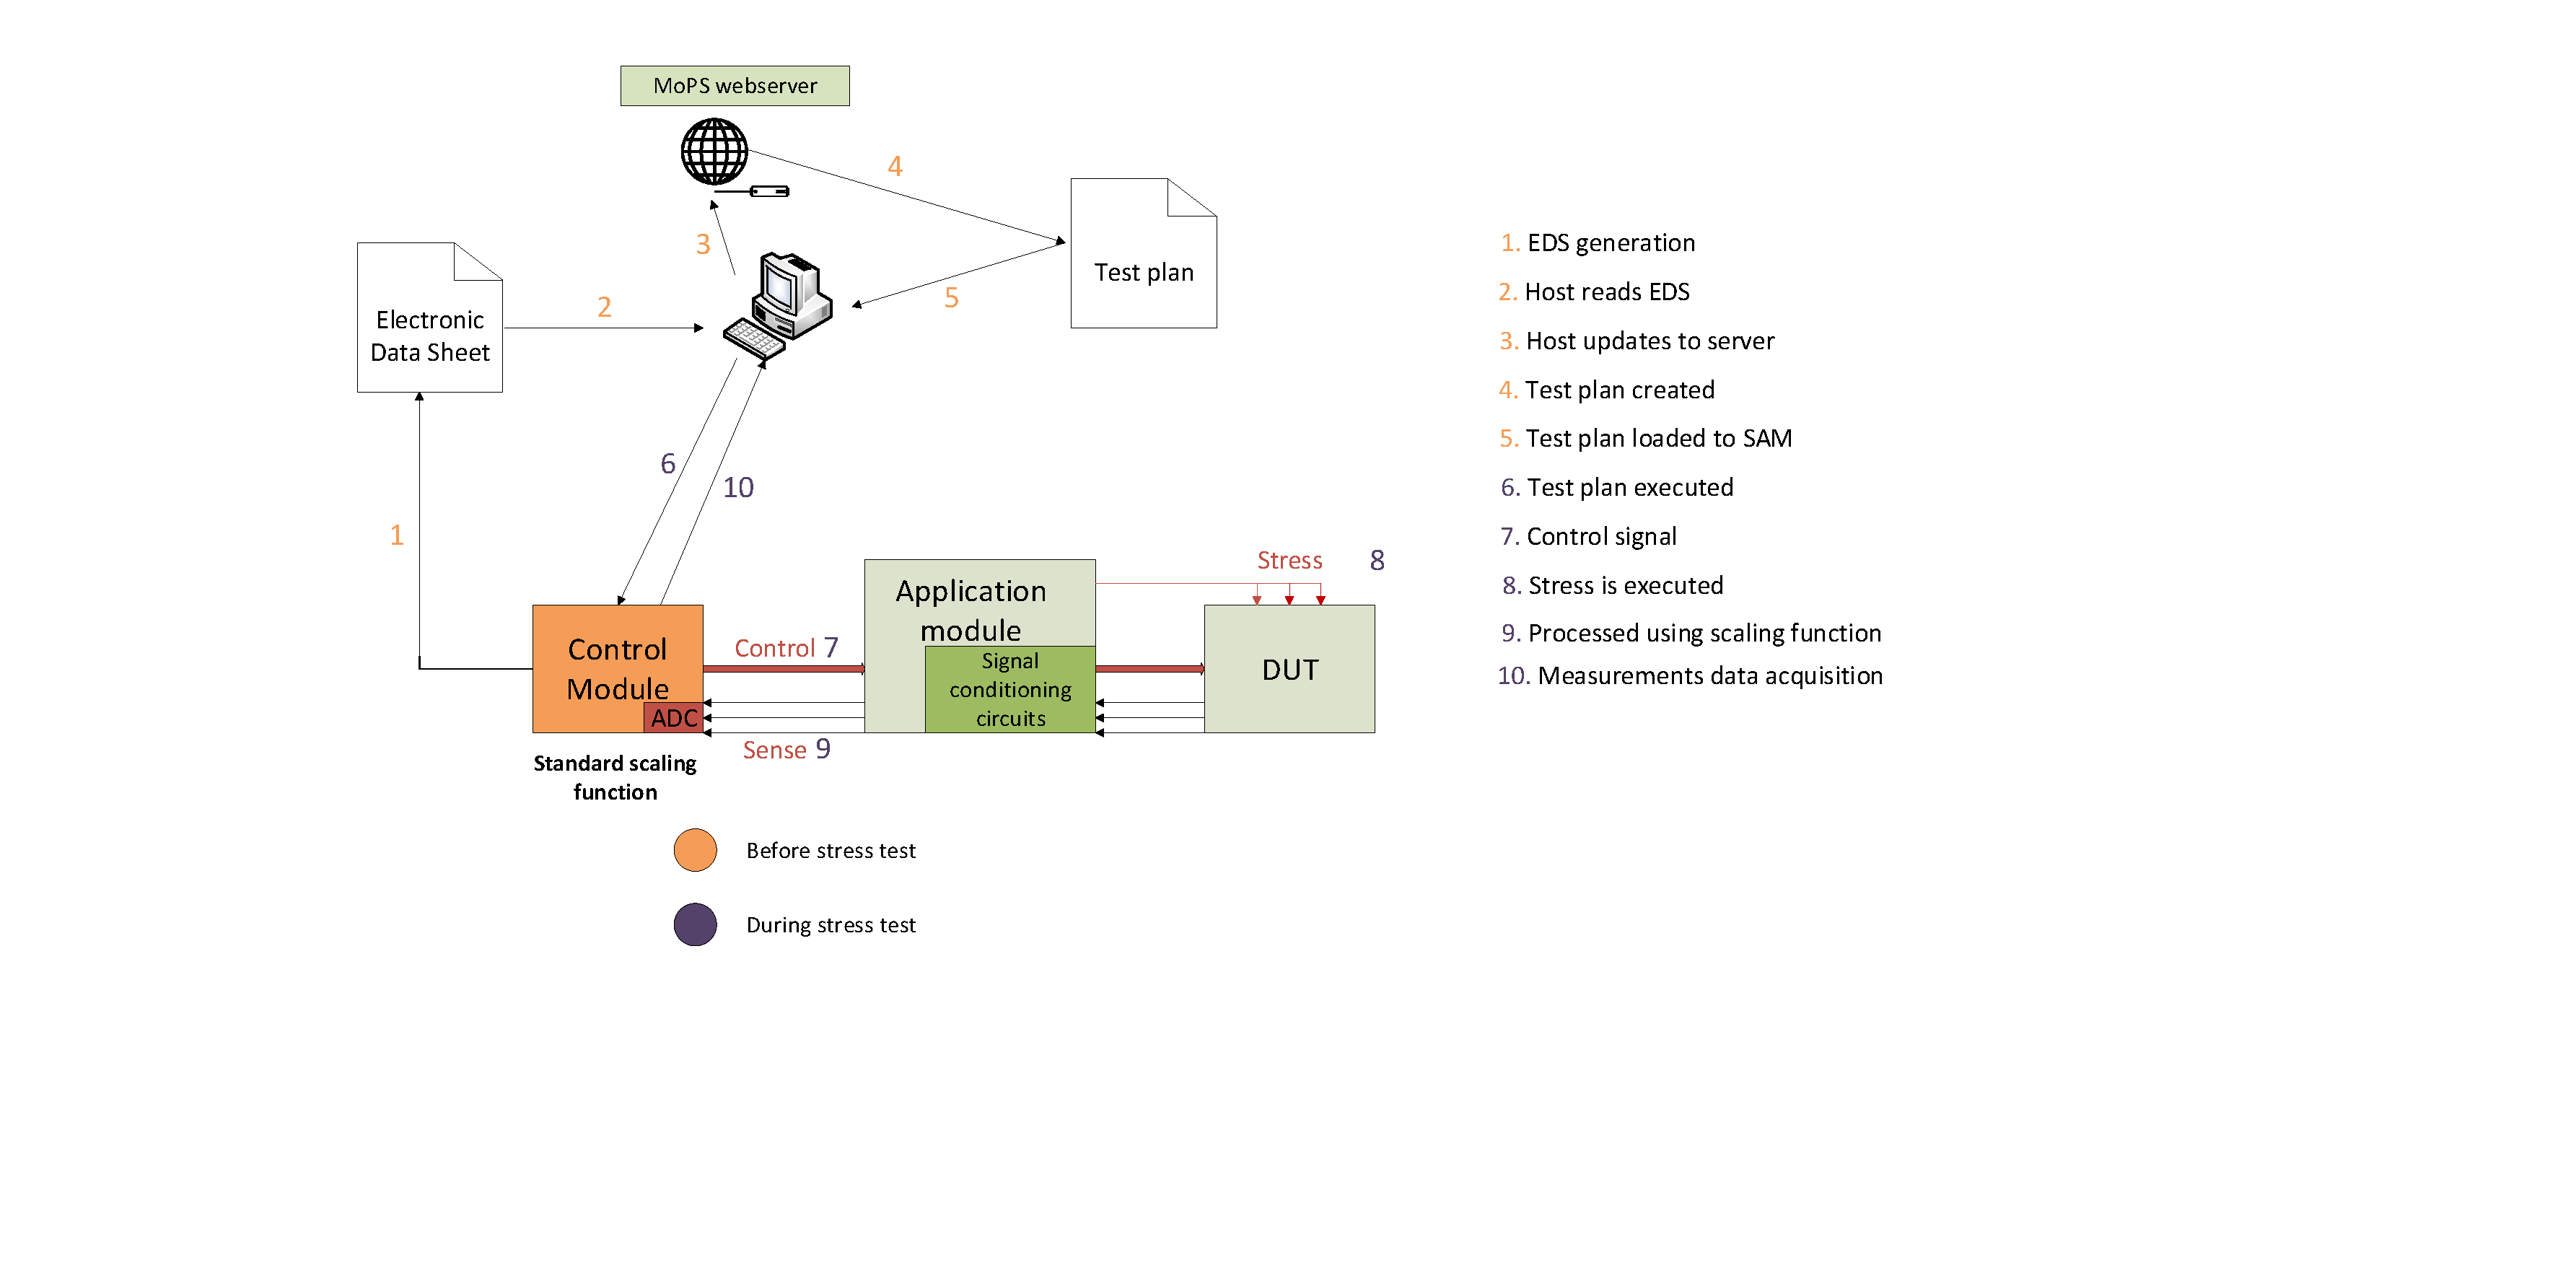
\includegraphics[trim=150 300 750 0, clip, width=\textwidth, scale=0.75]{images/Software_architecture.pdf}
		\caption{State of the art}
		\label{fig:SOA}
\end{figure}

\begin{enumerate}
\item The starting point of the stress test application is from the control module. A control module is flashed with a stress test application integrated firmware image to execute the test plan. Upon booting of microcontroller, an \acrshort{EDS} is generated in the MoPS CORE firmware project folder.
\item SAM accesses the latest \acrshort{EDS} that is generated in the MoPS CORE firmware project folder.
\item SAM further updates the latest EDS to MoPS web server.
\item Test plan builder tool downloads the EDS to create and validate the test plans that are created by test engineers.
\item A Semiconductor is not subjected to stress test until this point. SAM further keeps waiting to receive test plans to subject DUT into an application-specific stress test.
 Subsequently, Test plans (see \cref{sec:TP}) that are created by test engineers are loaded to SAM.
\item Test plans are forwarded by SAM to MicroMoPS for it's execution.
\item Test plans are executed and as a part of execution, the PWM signal is sent from the control Module to \acrshort{DUT}. 
The control (PWM) signal makes the DUT go into an operational mode.
\item Electrical stresses are applied onto DUT through the application module.
\item Electrical signals are generated in the DUT because of the electrical stresses that are exerted on the semiconductor device.
\item The generated electrical signals are measured through the analog communication channels of MicroMoPS.
\item The analog measurements are digitized using an ADC of MicroMoPS and the digitized values are later processed using a standard scaling function (see \cref{sec:ADC}) to convert them into discrete MicroMoPS specific voltage values.
\item The processed data are acquired by SAM to retain the original values of analog measurements. The retained values are used in the SAM for further interpretation such as, for calculating the end of life of DUT. 
\end{enumerate}     
